\chapter{Силы, кварки и первые адронные мультиплеты}

\section{Частицы, поля и недостающая третья сторона}

Волны представляют собой конфигурации полей, так что в нашем обсуждении эти два описания тесно связаны. Квантовая механика утверждает, что энергия в такой волне приходит дискретными, неделимыми порциями. Эти порции — её кванты, а кванты поля — это то, что мы называем его частицами. Имея в виду эту связь, мы уже обсудили волновые уравнения, принципы действия и общие свойства, переносимые частицами: энергию, импульс, спин и бозон--фермионное различие. Фермионы противятся занятию одного и того же состояния; бозоны могут собираться и конденсироваться в одном состоянии.

Квантовый лагранжиан также фиксирует взаимодействия. Произведения полей соответствуют вершинам, в которых частицы входят и выходят. Член, содержащий, например, четвёртую степень поля, представляет четырёхлучевую вершину взаимодействия. Так принцип действия превращается в компактный перечень возможных процессов с частицами.

Следующая задача — назвать частицы---не совсем по одной, а по семействам---и придать им некоторую индивидуальность: их свойства, их взаимодействия и их место в обычной физике. Однако прежде чем составить этот список, в одном концептуальном треугольнике всё ещё недостаёт одной стороны:
\begin{itemize}
\item частицы,
\item поля, квантами которых являются эти частицы,
\item силы, связанные с процессами обмена с участием тех же самых квантов.
\end{itemize}

Слово \emph{элементарный} пока должно оставаться предварительным. Любое правдоподобное определение элементарной, а не составной частицы в конце концов наталкивается на неоднозначный случай, и к этой проблеме мы ещё вернёмся. Пока же предположим, что фундаментальные поля существуют, и будем называть их кванты элементарными частицами. Если электрическое поле порождает электрические силы, а гравитационное поле — гравитационные силы, то и поле электрона тоже должно участвовать в силовых взаимодействиях. Треугольник может замкнуться, только если у силы есть описание не только в терминах поля, но и в терминах частиц.

Поэтому мы дважды выведем логику силы. Сначала воспользуемся классической энергией поля; затем спросим, как то же самое взаимодействие выглядит, когда поле разлагается на кванты. Лишь после того, как этот мост будет надёжно установлен, начнётся каталог частиц.

\section{Сила из энергии поля в классической электродинамике}

Поместим в пространстве два заряда. Один способ найти действующую между ними силу — сослаться на закон обратных квадратов. Более содержательный способ — спросить, что заряды делают с пространством: они создают электрические поля, а эти поля запасают энергию.

Полезно отделить каждый заряд от пространственной формы его поля,
\begin{equation}
\mathbf E_i=q_i\widehat{\mathbf E}_i,
\end{equation}
хотя от сохранения обозначения со шляпкой ничего не зависит. При наличии обоих зарядов линейность даёт
\begin{equation}
\mathbf{E}=\mathbf{E}_1+\mathbf{E}_2.
\end{equation}
С точностью до выбора единиц энергия электростатического поля имеет вид
\begin{equation}
U_{\text{field}}\propto\int d^3x\,\mathbf{E}^2.
\end{equation}
Подставляя сумму двух полей, получаем
\begin{align}
U_{\text{field}}
&\propto\int d^3x\,(\mathbf{E}_1+\mathbf{E}_2)^2 \\
&\propto\int d^3x\,\bigl(\mathbf{E}_1^2+\mathbf{E}_2^2
  +2\mathbf{E}_1\!\cdot\!\mathbf{E}_2\bigr).
\end{align}

Первые два члена — это собственные энергии. Перенос любого из зарядов переносит вместе с ним и его поле и не изменяет соответствующий интеграл. Эта энергия через \(E=mc^2\) вносит вклад в измеряемую массу изолированной заряженной частицы. То, как эта собственная энергия включается в измеряемую массу, относится к более поздней теме перенормировки. Никакая часть этой не зависящей от положения энергии не вносит вклада в силу между двумя частицами.

Перекрёстный член устроен иначе. Он не принадлежит отдельно ни одной из частиц и существует только тогда, когда присутствуют оба поля. Если разнести заряды очень далеко, области, где их поля заметны, почти не перекрываются. Когда заряды сближаются, перекрытие меняется. Поэтому энергия взаимодействия, зависящая от конфигурации, пропорциональна
\begin{equation}
U_{\text{int}}(r)\propto q_1q_2\int d^3x\,
\widehat{\mathbf E}_1\!\cdot\!\widehat{\mathbf E}_2.
\end{equation}
Для двух точечных зарядов, разделённых расстоянием \(r\), вычисление интеграла даёт привычную зависимость
\begin{equation}
U_{\text{int}}(r)\propto\frac{q_1q_2}{r}.
\end{equation}
Радиальная сила равна её отрицательному градиенту,
\begin{equation}
\mathbf F_{12}=-\boldsymbol\nabla_{\mathbf r}U_{\text{int}},
\qquad
|\mathbf F_{12}|\propto\frac{|q_1q_2|}{r^2}.
\end{equation}
\editorialnote{Устный аргумент отождествляет перекрёстный член с кулоновской силой, подчиняющейся закону обратных квадратов, не задерживаясь на потенциале. Стандартное промежуточное выражение \(U_{\mathrm{int}}\propto1/r\) здесь выписано явно, так что его градиент даёт указанную силу \(1/r^2\).}

Закон силы стал производной той части энергии поля, которая зависит от относительного положения. Когда два объекта далеко друг от друга, они фактически независимы. Если сблизить их, поле между ними перестраивается; возникающее изменение энергии и есть взаимодействие.

Но если поле можно разложить на кванты, на этом история не заканчивается. У той же самой силы должно быть и описание на языке частиц.

\section{Молекулярный обмен: два протона и один электрон}

Прежде чем вернуться к электродинамике, рассмотрим систему, в которой обмен легче себе представить: два протона и один электрон. Обмен — лишь один из нескольких источников молекулярных сил, но этот пример делает наглядной связь между обменом, энергией и силой. Он не предлагается как замена квантовой электродинамике.

Если присутствует один протон, а другой находится бесконечно далеко, электрон может занимать водородоподобное основное состояние с центром на первом протоне. Его волновая функция локализована вблизи этого силового центра.

\begin{figure}[h]
\centering
\includegraphics[width=0.72\textwidth]{lecture_01_figure_02.png}

\medskip

\begin{tikzpicture}[scale=0.95]
\draw (-0.2,0) -- (6.4,0);
\fill (1.3,0) circle (2pt);
\draw[smooth] plot coordinates {(0.1,0.15) (0.8,1.15) (1.5,1.75) (2.2,1.1) (3.0,0.35) (3.8,0.12)};
\node at (1.3,-0.35) {$p$};
\node at (2.7,1.55) {$\psi_1(x)$};
\end{tikzpicture}
\caption{Волновая функция водородоподобного основного состояния, локализованная около одного протона.}
\lectureframe{00:14:32}
\end{figure}
\editorialnote{Метка \(\psi_1(x)\) на перерисованном рисунке обозначает локализованный профиль, описанный в 00:14:30--00:14:32; она не скопирована с разборчивой подписи на доске.}

Теперь поместим второй протон на большое, но конечное расстояние. По симметрии существует второе локализованное состояние с той же одноцентровой энергией, на этот раз с центром на правом протоне.

\begin{figure}[h]
\centering
\includegraphics[width=0.78\textwidth]{lecture_01_figure_03.png}

\medskip

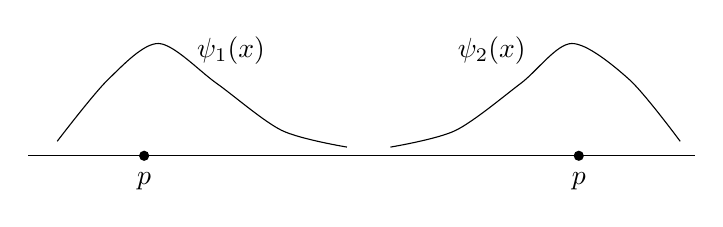
\begin{tikzpicture}[scale=0.92]
\draw (-0.2,0) -- (9.0,0);
\fill (1.4,0) circle (2pt);
\fill (7.4,0) circle (2pt);
\draw[smooth] plot coordinates {(0.2,0.2) (0.9,1.05) (1.6,1.55) (2.4,1.0) (3.3,0.35) (4.2,0.12)};
\draw[smooth] plot coordinates {(4.8,0.12) (5.7,0.35) (6.6,1.0) (7.3,1.55) (8.1,1.05) (8.8,0.2)};
\node at (1.4,-0.35) {$p$};
\node at (7.4,-0.35) {$p$};
\node at (2.6,1.45) {$\psi_1(x)$};
\node at (6.2,1.45) {$\psi_2(x)$};
\end{tikzpicture}
\caption{Два локализованных профиля, из которых составляется равновесная суперпозиция после того, как туннелирование становится возможным.}
\lectureframe{00:17:54}
\end{figure}
\editorialnote{Метки \(\psi_1(x)\) и \(\psi_2(x)\) обозначают два профиля, обсуждаемые в 00:17:41--00:17:56; эти символы представляют собой схематические метки, добавленные для наглядности.}

При бесконечном расстоянии между ними два состояния вырождены: локализация электрона слева или справа требует одной и той же энергии. При конечном расстоянии становится возможным новый процесс. Электрон может туннелировать через классически запрещённую область от одного центра к другому. Попытка проследить траекторию через барьер возмутила бы состояние; ``перескок'' — это описание квантовой эволюции, а не фильм классической траектории.

В равновесии вероятность обнаружить электрон вблизи любого из протонов одинакова. Поэтому нормировка даёт множитель \(1/\sqrt2\), и более низкое по энергии равновесное состояние приблизительно равно
\begin{equation}
\psi_+(x)\approx \frac{\psi_1(x)+\psi_2(x)}{\sqrt2}.
\end{equation}

Знак приближения здесь существен. Истинная двухцентровая волновая функция не является в точности суммой двух невозмущённых водородоподобных орбиталей; в области перекрытия она подстраивается. Для нас здесь важно, что симметричное равновесное состояние лежит ниже изолированной одноцентровой энергии. На языке гамильтониана левая и правая конфигурации связаны недиагональным матричным элементом. Если позволить электрону занимать их когерентную суперпозицию, энергия понижается.

\section{От понижения энергии к эффективной силе}

При большом расстоянии между протонами индуцированный электроном вклад \(E_e(r)\) стремится к своему значению для разделённых атомов. При меньшем расстоянии туннелирование и суперпозиция понижают его. Полный потенциал системы двух протонов--одного электрона должен также содержать прямое отталкивание протонов,
\begin{equation}
V_{\mathrm{tot}}(r)=V_{pp}(r)+E_e(r).
\end{equation}

Это вновь связывает молекулярный пример с рассуждением об энергии поля. Эскизы волновой функции и качественная кривая для \(E_e(r)\) — это два взгляда на один и тот же расчёт; равновесие определяется суммой \(V_{\mathrm{tot}}(r)\).

\begin{figure}[h]
\centering
\includegraphics[width=0.78\textwidth]{lecture_01_figure_04.png}

\medskip

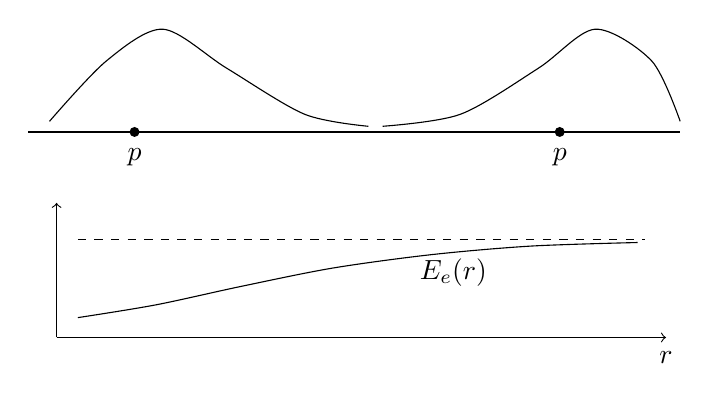
\begin{tikzpicture}[scale=0.9]
\draw (-0.2,3.0) -- (9.0,3.0);
\fill (1.3,3.0) circle (2pt);
\fill (7.3,3.0) circle (2pt);
\draw[smooth] plot coordinates {(0.1,3.15) (0.9,4.0) (1.7,4.45) (2.6,3.9) (3.7,3.25) (4.6,3.08)};
\draw[smooth] plot coordinates {(4.8,3.08) (5.9,3.25) (7.0,3.9) (7.8,4.45) (8.6,4.0) (9.0,3.15)};
\node at (1.3,2.65) {$p$};
\node at (7.3,2.65) {$p$};

\draw[->] (0.2,0.1) -- (0.2,2.0);
\draw[->] (0.2,0.1) -- (8.8,0.1);
\draw[dashed] (0.5,1.48) -- (8.5,1.48);
\draw[smooth] plot coordinates {(0.5,0.38) (1.6,0.56) (2.8,0.82) (4.1,1.08) (5.5,1.27) (6.9,1.39) (8.4,1.44)};
\node at (5.8,1.02) {$E_e(r)$};
\node at (8.8,-0.18) {$r$};
\end{tikzpicture}
\caption{Перекрытие волновых функций вверху и индуцированная электроном энергия внизу. При увеличении \(r\) она поднимается к асимптоте разнесённых атомов; полный потенциал протонов должен также включать их кулоновское отталкивание.}
\lectureframe{00:20:28}
\end{figure}
\editorialnote{Метки \(E_e(r)\) и \(r\) обозначают энергетическую кривую и расстояние, обсуждаемые в 00:19:12--00:20:38; сохранившийся кадр доски не позволяет разобрать эти подписи осей.}

Две соответствующие силы следуют из градиентов энергии,
\begin{equation}
F_{e}(r)=-\frac{dE_e}{dr},
\qquad
F_{\mathrm{tot}}(r)=-\frac{dV_{\mathrm{tot}}}{dr}.
\end{equation}
Тем самым система подталкивается к меньшей полной энергии. Там, где \(E_e(r)\) уменьшается при сближении протонов, обмен даёт притягивающий вклад; существует ли связанное расстояние, зависит от его конкуренции с \(V_{pp}(r)\). Это элементарный механизм, лежащий в основе ковалентной связи: электрон оказывается общим, потому что обобществлённое состояние энергетически выгодно.

В классическом расчёте перекрытие электрических полей изменяет энергию. Здесь два силовых центра допускают более низкое квантовое состояние. Оба механизма порождают силу, потому что равновесная энергия зависит от конфигурации.

Язык обмена можно подытожить схемой мировых линий. Ее нельзя понимать как наблюдаемую траекторию; она представляет амплитуды того, что электрон связан либо с одним, либо с другим протоном.

\begin{figure}[h]
\centering
\begin{tikzpicture}[scale=1.0]
\draw (0,0) -- (0,4.4);
\draw (4.8,0) -- (4.8,4.4);
\draw (0,0.9) .. controls (1.6,1.7) and (3.2,1.7) .. (4.8,2.5);
\draw (4.8,2.9) .. controls (3.2,2.1) and (1.6,2.1) .. (0,3.9);
\node at (0,-0.35) {$p$};
\node at (4.8,-0.35) {$p$};
\node at (2.35,1.55) {$e^-$};
\node at (2.35,2.55) {$e^-$};
\end{tikzpicture}
\caption{Обмен электроном между двумя мировыми линиями протонов, понимаемый как схема квантовых амплитуд, а не как наблюдаемая траектория.}
\end{figure}

\begin{classroomqa}
\audiencequestion{Можно ли понимать это притяжение просто как экранирование электроном протонного заряда или уменьшение его величины?\lecturetimestamp{00:23:26}}
\lecturerresponse{Нет. Уменьшение заряда — неправильная картина для этого эффекта. Существенный факт состоит в том, что сложение двух локализованных волновых функций дает состояние с немного меньшей энергией, чем каждое из локализованных состояний по отдельности.}
\end{classroomqa}

\begin{classroomqa}
\audiencequestion{Это ли имел в виду Фейнман, говоря, что ``свет любит свет''?\lecturetimestamp{00:23:51}}
\lecturerresponse{Нет. Эта фраза, скорее всего, относится к бозе-статистике: фотоны предпочитают общие состояния, тогда как электроны подчиняются запрету. Молекулярный эффект здесь — это туннелирование между двумя центрами.}
\end{classroomqa}

Два протона по-прежнему электростатически отталкиваются. Обмен имеет меньший радиус действия, чем кулоновское взаимодействие, поэтому нужно рассматривать полный потенциал, а не каждый из вкладов по отдельности. Тем не менее при подходящих расстояниях молекулярный ион \(\mathrm H_2^+\) связан; в нейтральной двухэлектронной системе дальнодействующее зарядовое отталкивание отсутствует, и ковалентное связывание там еще более привычно.

\begin{classroomqa}
\audiencequestion{Главный ли эффект помещения электрона между протонами состоит в уменьшении их электростатического отталкивания?\lecturetimestamp{00:24:33}}
\lecturerresponse{Это немного уменьшает отталкивание, но не в этом состоит главный эффект. Обмен электроном — сила с меньшим радиусом действия, чем кулоновское отталкивание. Он наиболее заметен в нейтральной двухэлектронной системе, где дальнодействующая электростатическая сила между атомами отсутствует, но туннелирование все еще порождает притяжение.}
\end{classroomqa}

\begin{classroomqa}
\audiencequestion{Действительно ли положительно заряженный молекулярный ион \(\mathrm H_2^+\), имеющий только один электрон, связан?\lecturetimestamp{00:26:06}}
\lecturerresponse{Да. При достаточно малом расстоянии обменное притяжение достаточно сильно, чтобы преодолеть кулоновское протон--протонное отталкивание.}
\end{classroomqa}

\begin{classroomqa}
\audiencequestion{Создает ли двухцентровая конфигурация третью силу?\lecturetimestamp{00:26:24}}
\lecturerresponse{Нет, никакая новая фундаментальная сила не вводится. Уравнение Schr\"odinger в суммарном потенциале двух протонов имеет равновесную энергию, отличную от энергии в одноцентровой задаче; производная этой измененной энергии и есть эффективная сила.}
\end{classroomqa}

\begin{classroomqa}
\audiencequestion{Является ли понижение энергии примером квантовой запутанности?\lecturetimestamp{00:27:06}}
\lecturerresponse{Не в обычном двухчастичном смысле: нужен только один электрон. Существенной математической особенностью здесь является внедиагональный матричный элемент гамильтониана, связывающий левое и правое состояния.}
\end{classroomqa}

\begin{classroomqa}
\audiencequestion{Что происходит с обменом при высокой температуре?\lecturetimestamp{00:27:37}}
\lecturerresponse{При экстремально высокой температуре электрон ионизуется и совсем забывает о молекуле. При меньшей энергии возбуждения он может занять более протяженную орбиталь, изменяя перекрывание и, следовательно, силу. Это зависящая от состояния поправка, а не новый общий механизм.}
\end{classroomqa}

\section{Обмен фотонами и первые записи таблицы}

Можно ли описать кулоновскую силу на том же языке обмена? Заряженная частица взаимодействует с электромагнитным полем, кванты которого — фотоны. Классически мы находим электрическое поле вокруг заряда. В квантовой теории поля мы разлагаем это взаимодействие на испускание и поглощение фотонов.

Физическая заряженная частица — это не просто голый заряд. Ее состояние представляет собой квантовую суперпозицию, содержащую компоненту голого электрона, электрона с одним фотоном, электрона с двумя фотонами и так далее. В намеренно схематической записи,
\begin{equation}
\begin{aligned}
\ket{e_{\mathrm{phys}}}
={}&a_0\ket e
+a_1\ket{e+\text{one photon}}
\\
&+a_2\ket{e+\text{two photons}}+\cdots .
\end{aligned}
\end{equation}
Эта запись отражает только иерархию компонент с разным числом фотонов; она не задает импульсов фотонов и не претендует на полное построение взаимодействующего заряженного состояния.
Окружающие фотоны испускаются и вновь поглощаются, а не уходят как свободное излучение. Их эффекты можно измерить, хотя детектируют их не так, как свободно распространяющиеся фотоны. Если поместить рядом второй заряд, фотон, испущенный одним зарядом, может быть поглощен другим. Тогда энергия этих двух одетых состояний перестает быть равной простой сумме двух изолированных энергий.

Аудиторная аналогия — это два жонглера, каждый со своим набором мячей. Когда они далеко друг от друга, каждый жонглирует независимо. Стоит подвести их достаточно близко, и один может поймать мяч, брошенный другим. На языке диаграмм Фейнмана этот общий объект — обмениваемый фотон. Аналогия не изображает микроскопическую траекторию, но передает, почему близость делает возможным новый процесс.

Теперь у нас есть два описания, выходящие за рамки простого заучивания закона Кулона. Классическая теория поля складывает поля и возводит результат в квадрат. Квантовая теория поля суммирует амплитуды, в которых обмениваются кванты. В этом смысле частицы, поля и силы образуют взаимно-однозначное соответствие. Электроны опосредуют молекулярный обмен, фотоны — электромагнитный обмен, и любая частица, которой можно обмениваться, может в подходящей ситуации вносить вклад в силу. Поэтому привычное утверждение, что в природе есть 4 фундаментальных взаимодействия, является классификацией на более широком уровне; в рамках языка обмена каждый вид частиц, которым может идти обмен, может порождать собственный вклад в эффективную силу.

Наконец пришло время назвать частицы, перечислить их свойства и сказать, в каких процессах они могут участвовать. Если выписать всю стандартную модель сразу, получится лишь длинная проверка памяти, поэтому мы разобьем частицы на небольшие группы, члены которых просто связаны друг с другом, и разберем, что может делать каждая группа.

Полный каталог громоздок, потому что мы не понимаем, почему существуют именно эти частицы, тогда как другие мыслимые частицы не существуют. Математическая согласованность задает некоторые связи: если существует несколько членов некоторой схемы, для ее завершения может потребоваться еще один. Эти связи уменьшают число независимых фактов, но лишь в умеренной степени. Многие типы частиц и многие параметры остаются необъясненными. Понимание этой незавершенной структуры необходимо, чтобы понять, что пытаются обнаружить последующие эксперименты.

\begin{figure}[h]
\centering
\includegraphics[width=0.7\textwidth]{lecture_01_figure_05.png}
\caption{Первая запись в таблице частиц обозначает фотон символом \(\gamma\), а его поле — векторным потенциалом \(A\).}
\lectureframe{00:39:11}
\end{figure}

Первое соответствие поле--квант имеет вид
\begin{equation}
\gamma \leftrightarrow A.
\end{equation}
Здесь \(A\) — электромагнитный векторный потенциал. Фотон — бозон со спином 1, нулевым электрическим зарядом, нулевым барионным числом и нулевой массой покоя. Электронное поле принято обозначать \(\psi_e\); его компоненты рождения и уничтожения действуют на состояния электрона и позитрона.

В нашей таблице указаны название, символ частицы, поле, тип — бозон или фермион, электрический заряд \(Q\), барионное число \(B\) и масса:

\begin{table}[h]
\centering
\resizebox{\linewidth}{!}{%
\begin{tabular}{lllllll}
Название & Символ & Поле & Тип & \(Q\) & \(B\) & Масса \\
Фотон & \(\gamma\) & \(A\) & бозон & \(0\) & \(0\) & \(0\) \\
Электрон & \(e^-\) & \(\psi_e\) & фермион & \(-1\) & \(0\) & \(0.51\,\mathrm{MeV}\) \\
Позитрон & \(e^+\) & \(\psi_e\) & фермион & \(+1\) & \(0\) & \(0.51\,\mathrm{MeV}\)
\end{tabular}
}%
\caption{Записи для фотона и электрона--позитрона, которыми начинается каталог частиц.}
\end{table}

Электрон и позитрон связаны взаимно: каждый является античастицей другого. Называть отрицательно заряженное состояние ``частицей'' — условность. Электрический заряд измеряют в единицах модуля заряда электрона, поэтому
\begin{equation}
Q(e^-)=-1,\qquad Q(e^+)=+1.
\end{equation}
Массу измеряют в единицах энергии, используя \(E=mc^2\). Один электрон-вольт — это энергия, приобретаемая зарядом \(e\) при прохождении разности потенциалов в один вольт,
\begin{equation}
1\,\mathrm{eV}=e\,(1\,\mathrm V).
\end{equation}
Эта единица естественно возникает в атомной физике: в качестве грубой атомной шкалы ионизация водорода требует примерно \(13.5\,\mathrm{eV}\). Для масс частиц нужны миллионы или миллиарды электрон-вольт. Масса электрона равна
\begin{equation}
m_e c^2 \approx 0.511\,\mathrm{MeV}.
\end{equation}

\begin{classroomqa}
\audiencequestion{Должна ли масса электрона быть в точности равна половине МэВ?\lecturetimestamp{00:44:02}}
\lecturerresponse{Нет. Удобное округленное значение \(0.51\,\mathrm{MeV}\) не фиксируется никаким принципом как точная половина; это измеряемый параметр.}
\end{classroomqa}

В элементарном процессе КЭД одна линия заряженного фермиона входит, одна выходит, и к ним присоединена одна фотонная линия. Перестановка или кроссинг внешних линий позволяет той же вершине описывать испускание фотона, его поглощение или процесс с позитроном. В используемой здесь нековариантной схематической записи взаимодействие содержит
\begin{equation}
\mathcal{L}_{\mathrm{int}}\sim e\,\psi_e^\dagger \psi_e A.
\end{equation}
Разложение полей по операторам рождения и уничтожения даёт члены, которые уничтожают входящий электрон, создают выходящий электрон и создают или уничтожают фотон. Константа связи \(e\) даёт в вершине один множитель. Поэтому при испускании фотона, когда электрон рассеивается или ускоряется,
\begin{equation}
\mathcal{A}_{\mathrm{vertex}}\propto e,
\qquad
P_{\mathrm{emission}}\propto e^2.
\end{equation}
Один из практических случаев, где важна эта вероятность испускания фотона, — когда электрон попадает в мишень в рентгеновской трубке. Повторные сочетания той же вершины порождают процессы квантовой электродинамики, включая сдвиг энергии, интерпретируемый как сила между зарядами.

Поэтому такая схематическая вершина полезна.

\begin{figure}[h]
\centering
\begin{tikzpicture}[scale=1.0]
\fill (0,0) circle (1.5pt);
\draw (-1.6,-1.2) -- (0,0) -- (1.6,-1.2);
\draw (0,0) -- (0,1.8);
\node at (-1.8,-1.4) {$e^-$};
\node at (1.8,-1.4) {$e^-$};
\node at (0.35,1.95) {$\gamma$};
\end{tikzpicture}
\caption{Топологическая схема элементарной вершины КЭД: одна линия заряженного фермиона входит, одна выходит, и присоединён один фотон. Прямая фотонная линия здесь служит лишь упрощённым условным изображением.}
\end{figure}

Обменный вклад в силу связывает две такие вершины:

\begin{figure}[h]
\centering
\begin{tikzpicture}[scale=1.0]
\draw (0,0) -- (0,4.0);
\draw (4.8,0) -- (4.8,4.0);
\draw (0,2.0) -- (4.8,2.0);
\node at (0,-0.35) {$e^-$};
\node at (4.8,-0.35) {$e^-$};
\node at (2.4,2.3) {$\gamma$};
\end{tikzpicture}
\caption{Топологическая схема обмена фотоном, дающая квантово-полевое описание кулоновского взаимодействия.}
\end{figure}

Теперь, когда треугольник частица--поле--сила замкнут, можно продолжить каталог.

\section{Кварки, барионное число и загадка семейств}

Если бы этот каталог составлялся около 1960 года, за электронами и фотонами, вероятно, шли бы протоны и нейтроны. В современной физике элементарных частиц сначала вводят кварки. В наивной картине составляющих протоны и нейтроны представляют собой сравнительно большие составные объекты, построенные из более мелких кварковых степеней свободы. Точный смысл слова \emph{составной} ещё предстоит выяснить, но язык составляющих уже чрезвычайно полезен.

Все кварки — фермионы. Они несут барионное число, величину, введённую в ядерной физике при подсчёте нуклонов. \emph{Нуклон} означает конкретно протон или нейтрон. \emph{Барион} — более широкий класс, включающий нуклоны и похожие тяжёлые частицы, которые встретятся далее. Протон и нейтрон имеют по одной единице,
\begin{equation}
B(p)=B(n)=1,
\qquad
B(\bar p)=B(\bar n)=-1.
\end{equation}
Для ядра этот счёт барионов в точности совпадает с массовым числом \(A=Z+N\), то есть с числом протонов плюс нейтронов. Численное значение атомной массы, измеренной в атомных единицах массы, лишь приблизительно равно \(A\). В бета-процессах протоны могут превращаться в нейтроны, а нейтроны — в протоны, но общее число нуклонов не меняется. Например,
\begin{equation}
n\longrightarrow p+e^-+\bar\nu_e
\end{equation}
изменяет числа протонов и нейтронов по отдельности, сохраняя их сумму.

\begin{classroomqa}
\audiencequestion{Противоречат ли изотопы сохранению суммы числа протонов и нейтронов?\lecturetimestamp{00:52:03}}
\lecturerresponse{В разных изотопах действительно содержится разное число нейтронов, и бета-распад может превращать нейтрон в протон и наоборот. В обычном ядерном процессе сохраняющейся величиной является полное барионное число, а не число частиц каждого из этих видов по отдельности.}
\end{classroomqa}

Нормировка условна. Мы могли бы приписать протону барионное число \(2\), \(7\) или \(\pi\), если бы каждая составная частица масштабировалась согласованно. После того как протону приписано \(B=1\) и он содержит 3 кварка, каждый кварк должен нести
\begin{equation}
B(q)=\frac13,
\qquad
B(\bar q)=-\frac13.
\end{equation}
Таким образом, дробное значение является историческим следствием того, что сначала нормировали составной нуклон.

\begin{classroomqa}
\audiencequestion{Сохраняется ли число кварков?\lecturetimestamp{00:54:23}}
\lecturerresponse{Пары кварк--антикварк могут рождаться и уничтожаться, так что само по себе это число не сохраняется. Величина, соответствующая барионному числу, — это число кварков минус число антикварков, делённое на 3. Эмпирически она сохраняется с чрезвычайно высокой точностью, хотя здесь не предполагается, что это абсолютный закон.}
\end{classroomqa}

Гипотетический распад с сохранением заряда, такой как
\begin{equation}
p\longrightarrow e^++\gamma
\end{equation}
переводил бы барионное число 1 в конечное состояние с нулевым барионным числом. Этот канал приведён лишь как иллюстративный пример учёта, а не как предлагаемая модель распада. Ни одного процесса с нарушением барионного числа не наблюдалось. Приведённая здесь грубая граница помещает время жизни протона как минимум в диапазон \(10^{33}\)--\(10^{34}\) лет. Никто не наблюдает один-единственный протон так долго; наблюдают огромное число протонов в течение приемлемого времени, компенсируя длительность жизни размером выборки. Тем не менее распад протона широко ожидался, и ничто в обсуждаемой здесь математике не давало абсолютного запрета. Поэтому вопрос о том, сохраняется ли барионное число в точности, оставался открытым экспериментальным вопросом: нарушений не наблюдали, ограничения были жёсткими, но возможность не отвергалась.

\begin{classroomqa}
\audiencequestion{Нарушает ли аннигиляция протон--антипротон барионное число?\lecturetimestamp{00:56:17}}
\lecturerresponse{Нет. Начальное барионное число равно \(1+(-1)=0\), так что аннигиляция в конечное состояние с нулевым барионным числом его сохраняет. Нарушением был бы распад одиночного протона в небарионные продукты.}
\end{classroomqa}

Существует 6 ароматов кварков,
\begin{equation}
u,\ d,\ s,\ c,\ b,\ t,
\end{equation}
называемых up, down, strange, charm, bottom и top. В up-кварке нет ничего направленного вверх, а strange-кварк ничуть не страннее своих соседей; эти названия отражают историю, а не логику. Обозначения полей не вполне единообразны: и для поля, и для его кванта можно встретить \(q\), \(Q\), \(\psi_q\) или просто букву аромата \(u,d,s,c,b,t\).

\begin{classroomqa}
\audiencequestion{Являются ли bottom и top теми же частицами, которые когда-то называли beauty и truth?\lecturetimestamp{00:58:35}}
\lecturerresponse{Да. Менее вычурные названия bottom и top стали стандартными. История именования не несёт динамического содержания.}
\end{classroomqa}

Их электрические заряды повторяются тремя парами:
\begin{equation}
\begin{aligned}
Q(u)=Q(c)=Q(t)&=+\frac23,
\\
Q(d)=Q(s)=Q(b)&=-\frac13.
\end{aligned}
\end{equation}
Антикварки несут противоположные значения как электрического заряда, так и барионного числа. Изолированный дробный заряд никогда не наблюдается, потому что кварки не встречаются как свободные асимптотические частицы; наблюдаемые адроны имеют целый электрический заряд.

Пары \((d,u)\), \((s,c)\) и \((b,t)\) образуют 3 семейства, повторяющие одну и ту же схему зарядов. Все шесть по-прежнему несут \(B=1/3\).

\begin{classroomqa}
\audiencequestion{Несут ли более тяжёлые кварки также барионное число \(1/3\)?\lecturetimestamp{01:02:02}}
\lecturerresponse{Да. Каждый кварк несёт барионное число \(1/3\).}
\end{classroomqa}

Массы не показывают никакой сопоставимой повторяемости. Полезные оценки порядка величины таковы:
\begin{align}
m_u &\sim 5\,\mathrm{MeV},
&
m_d &\sim 10\,\mathrm{MeV},
\\
m_s &\sim 100\,\mathrm{MeV},
&
m_c &\sim 10^3\,\mathrm{MeV},
\\
m_b &\sim 5\,\mathrm{GeV},
&
m_t &\sim 170\,\mathrm{GeV}.
\end{align}
Здесь \(1\,\mathrm{GeV}=10^3\,\mathrm{MeV}\); переход к другой единице делает значения для bottom- и top-кварков удобочитаемыми. Оценка массы down-кварка намного больше, чем у электрона \(0.511\,\mathrm{MeV}\), но намного меньше, чем у протона, примерно \(940\,\mathrm{MeV}\), то есть около \(1{,}800\) масс электрона. Действительно, если сложить 2 лёгких значения для up-кварка и 1 значение для down-кварка, до массы протона всё равно очень далеко; оставшуюся часть энергии адрона в конечном счёте ещё предстоит объяснить.

\editorialnote{В устном сравнении down-кварк с массой \(10\,\mathrm{MeV}\) был назван примерно пятьюдесятью массами электрона. При приведённых здесь грубых значениях \(10/0.511\approx20\); иерархия верна, но множитель пятьдесят — арифметическая ошибка.}

Даже порядок внутри пары не повторяется: down-кварк тяжелее up-кварка, тогда как charm-кварк гораздо тяжелее strange-кварка. top-кварк в десятки тысяч раз тяжелее up-кварка, хотя их заряды и характер взаимодействий весьма близки.

Здесь на самом деле две загадки. Мы не понимаем, почему существует хотя бы одно семейство кварков, хотя первое семейство по крайней мере даёт up- и down-кварки, необходимые для протонов, нейтронов и обычного вещества. Мы также не понимаем, почему природа повторяет эту схему во втором и третьем семействах и почему массы повторяющихся частиц разбросаны по столь многим порядкам величины. Идеи есть, но принятого объяснения, которое вычисляло бы эту схему, нет.

\begin{classroomqa}
\audiencequestion{Если масса top-кварка не имеет фундаментального объяснения, как её приблизительное значение удавалось оценить до прямого открытия?\lecturetimestamp{01:05:53}}
\lecturerresponse{Эта оценка не выводила массу из более глубокого принципа. Предполагают пробное значение массы, вычисляют диаграммы, в которых виртуальные top-кварки влияют на хорошо измеренные процессы, и спрашивают, какое значение согласуется с этими наблюдениями. Косвенная чувствительность может локализовать параметр, не объясняя, почему природа выбрала именно его.}
\end{classroomqa}

\begin{classroomqa}
\audiencequestion{Если свободный кварк нельзя изолировать, в каком смысле можно обнаружить кварк?\lecturetimestamp{01:08:04}}
\lecturerresponse{Обнаружимы свидетельства существования кварков: их рождение оставляет характерные энергии, направления и струи частиц, а виртуальные кварки влияют на другие наблюдаемые величины. Невозможно приготовить одиночный кварк, отделённый от всех адронных спутников, и исследовать его как изолированную асимптотическую частицу.}
\end{classroomqa}

\begin{classroomqa}
\audiencequestion{Выводится ли схема зарядов \(-1/3\) и \(+2/3\) из теории, или это лишь способ учёта?\lecturetimestamp{01:09:02}}
\lecturerresponse{Часть этой схемы требуется математической непротиворечивостью, но лишь часть. На данном этапе заряды просто фиксируются как факты; условия непротиворечивости будут обсуждаться только после того, как будет введена большая часть Стандартной модели.}
\end{classroomqa}

В обычном веществе заметную распространённость имеют только кварки \(u\) и \(d\). Более тяжёлые ароматы распадаются к более лёгким состояниям. Поэтому относительная распространённость u- и d-кварков определяется главным образом космической и ядерной распространённостью протонов и нейтронов, а также их составом.

\begin{classroomqa}
\audiencequestion{Что определяет относительную распространённость шести кварковых ароматов во Вселенной?\lecturetimestamp{01:09:49}}
\lecturerresponse{Устойчивое вещество по существу содержит u- и d-кварки; более тяжёлые ароматы распадаются. Свободные нейтроны распадаются, тогда как протоны устойчивы на наблюдаемых временах, хотя нейтроны остаются распространёнными, когда связаны в ядрах. Поэтому подсчёт u- и d-кварков на этом уровне сводится к подсчёту этих протонов и нейтронов.}
\end{classroomqa}

\section{От кварков к адронам: нуклоны, странные барионы и мезоны}

После того как заряды кварков известны, можно вновь построить знакомые адроны. И нейтрон, и протон содержат по три валентных кварка,
\begin{equation}
n=ddu,
\qquad
p=uud.
\end{equation}
Их заряды сразу легко проверить:
\begin{align}
Q(n) &= Q(d)+Q(d)+Q(u)
= -\frac13-\frac13+\frac23
=0,\\
Q(p) &= Q(u)+Q(u)+Q(d)
= \frac23+\frac23-\frac13
=1.
\end{align}

На мгновение забудем о фотонах. Если выключить электромагнетизм, протон и нейтрон выглядят почти как один и тот же объект при взаимной замене \(u\) и \(d\). Эта почти симметрия не является точной, потому что массы двух кварков не совсем одинаковы. Мы дадим этой симметрии название и разовьём её только после знакомства с соответствующими лёгкими мезонами.

Поскольку \(m_d>m_u\), нейтрон, содержащий два d-кварка, должен получать больший вклад от кварковых масс. Электромагнитная самоэнергия действует в противоположную сторону: заряженный протон запасает энергию электрического поля, тогда как нейтрон не имеет суммарного заряда. В природе это соревнование разрешается тем, что нейтрон оказывается немного тяжелее. На этом грубом уровне приближения
\begin{align}
m_pc^2&\approx940\,\mathrm{MeV},\\
m_nc^2&\approx940\,\mathrm{MeV},\\
(m_n-m_p)c^2&\approx1.4\,\mathrm{MeV}.
\end{align}

\begin{classroomqa}
\audiencequestion{Каковы массы протона и нейтрона?\lecturetimestamp{01:15:35}}
\lecturerresponse{Обе близки к \(940\,\mathrm{MeV}\), а разность на этом грубом уровне составляет около \(1.4\,\mathrm{MeV}\).}
\end{classroomqa}

Тем не менее этого небольшого превышения достаточно, чтобы был возможен распад свободного нейтрона. После вычета энергии покоя электрона оставшаяся энергия может проявиться как кинетическая энергия в процессе \(n\to p+e^-+\bar\nu_e\).

Та же логика по составляющим приводит и к странным барионам. Поскольку \(s\) и \(d\) имеют одинаковый электрический заряд, d-кварк можно заменить на s-кварк, не меняя схему зарядов:
\begin{equation}
uds,\qquad uss,\qquad uus.
\end{equation}
Таким образом, \(uds\) и \(uss\) в приведённых выше примерах нейтральны, тогда как \(uus\) имеет заряд \(+1\). Такие состояния получили названия, в том числе \(\Lambda\) и \(\Xi\); на данном этапе подробное сопоставление этих названий не требуется. Замена \(d\) на \(s\) качественно аналогична замене одного вида нуклона другим в аналогичном ядре: значительная часть картины связывания сохраняется, тогда как изменение составляющей сдвигает массу. Эти состояния тяжелее обычных нуклонов и распадаются на более лёгкие барионы вместе с теми дополнительными частицами, которые необходимы, чтобы унести энергию и другие сохраняющиеся квантовые числа.

\begin{classroomqa}
\audiencequestion{Что появляется при распаде странного бариона?\lecturetimestamp{01:19:02}}
\lecturerresponse{Появляется более лёгкий барион, такой как протон или нейтрон, но он не может быть единственным продуктом: избыток энергии и сохраняющиеся квантовые числа требуют дополнительных частиц. Подробные правила распада откладываются.}
\end{classroomqa}

Подробные правила замены сложнее, чем этот первый перечень, но одна надёжная операция состоит в замене одного аромата другим с тем же электрическим зарядом. Замена d-кварка на s-кварк добавляет примерно \(90\,\mathrm{MeV}\) на этом грубом уровне по составляющим. Поэтому эти барионы несколько тяжелее протонов и нейтронов. Поскольку они могут распадаться на более лёгкие нуклоны, в обычном веществе и в окружающем нас космосе они не распространены.

\begin{classroomqa}
\audiencequestion{Есть ли у каждого бариона антибарион, получаемый заменой каждого кварка на его антикварк?\lecturetimestamp{01:20:33}}
\lecturerresponse{Да. Замена каждой составляющей на её античастицу даёт антипротон, антинейтрон или соответствующий антистранный барион, причём все аддитивные заряды меняют знак на противоположный.}
\end{classroomqa}

\begin{classroomqa}
\audiencequestion{Что будет, если вместо этого заменить strange-кварк на bottom-кварк?\lecturetimestamp{01:21:00}}
\lecturerresponse{В результате получится bottom-барион. ``Странный барион'' конкретно означает, что присутствует кварк \(s\); это прилагательное называет аромат, а не общую степень непривычности.}
\end{classroomqa}

Прилагательное \emph{странный} возникло после того, как физики уже освоились с протонами и нейтронами, и вновь открытые частицы казались неожиданными рядом с ними. Когда ароматическая структура известна, их существование не более странно, чем существование любого другого кваркового композита.

Массы составляющих выявляют важное предостережение. Если сложить две массы u-кварка и одну массу d-кварка, получится лишь несколько десятков МэВ, что и близко не подходит к примерно \(940\,\mathrm{MeV}\) у протона. В этой наивной сумме отсутствует нечто существенное. Протон и нейтрон также содержат глюоны, а глюоны несут энергию. В релятивистской связанной системе масса композита не получается простым сложением перечисленных масс его составляющих.

\begin{classroomqa}
\audiencequestion{Откуда берётся кажущаяся недостающей масса протона и нейтрона? Имеют ли глюоны массу?\lecturetimestamp{01:21:26}}
\lecturerresponse{В рамках этого учёта глюоны не несут барионного числа, но они несут энергию. Их энергия и составляет часть причины того, почему масса протона или нейтрона не равна сумме указанных масс лёгких кварков.}
\end{classroomqa}

\begin{classroomqa}
\audiencequestion{Является ли этот недостающий вклад формой энергии связи?\lecturetimestamp{01:22:03}}
\lecturerresponse{Да, его можно назвать формой энергии связи. Предостережение состоит в том, что массы релятивистских композитов не складываются тем простым образом, который подсказывает сложение параметров масс составляющих.}
\end{classroomqa}

\begin{classroomqa}
\audiencequestion{Можно ли описывать составной протон на языке полей так же, как и на языке частиц?\lecturetimestamp{01:22:45}}
\lecturerresponse{Да, но это намного труднее. Для развиваемого здесь учёта по составляющим язык частиц гораздо прозрачнее, чем попытка непосредственно комбинировать пространственно протяжённые поля.}
\end{classroomqa}

\begin{classroomqa}
\audiencequestion{Обычная энергия связи отрицательна относительно разделённых составляющих. Почему динамический вклад нуклона представляет собой большую положительную энергию?\lecturetimestamp{01:23:32}}
\lecturerresponse{Обычная интуиция об отрицательной энергии связи здесь неверна. Объяснение относится к более позднему изложению сильного взаимодействия, так что пока этот вопрос откладывается.}
\end{classroomqa}

Почему три кварка образуют барионы, тогда как два кварка не образуют изолированный двухкварковый адрон? В ранние годы кварковой теории это была настоящая загадка. Можно было бы ответить, что наблюдаемые связанные комбинации должны иметь электрический заряд, равный целому кратному заряда электрона. Само по себе это звучит как порочный круг: это описывает закономерность, не объясняя её. Тем не менее правило оказалось указанием в правильном направлении, а его более глубокое происхождение можно понять только после того, как будет введена большая часть сильного взаимодействия. Пока же это явно рабочее правило: три кварка могут образовать барион, тогда как кварк и антикварк могут образовать мезон, и получающиеся наблюдаемые композиты имеют целочисленный заряд.

Барионы, составленные из трёх одинаковых лёгких ароматов, тоже встречаются, но их детали могут подождать до обсуждения мезонов.

Мезоны — это композиты \(q\bar q\). Их барионное число равно нулю,
\begin{equation}
B(q\bar q)=\frac13-\frac13=0.
\end{equation}
В самых лёгких примерах используются \(u\) и \(d\). Эти ароматы намного легче остальных, устойчивы или исчезают в обычном веществе сравнительно медленно и широко представлены в природе. Их низкий порог рождения также означает, что в столкновениях они возникают легче, чем тяжёлые ароматы. По всем этим причинам композиты из лёгких кварков были первыми мезонами, с которыми столкнулись экспериментально, и именно с них естественно начать.

Естественный базис по аромату имеет вид
\begin{equation}
\ket{\bar u d},\qquad \ket{u\bar d},\qquad \ket{\bar u u},\qquad \ket{\bar d d}.
\end{equation}
В этом первом подсчёте никакого дополнительного ограничения не вводится: сохраняются все четыре лёгкие пары кварк--антикварк, и затем вычисляются их электрические заряды.

Заряженные состояния получаются сразу. Поскольку \(Q(\bar u)=-2/3\) и \(Q(d)=-1/3\),
\begin{align}
Q(\bar u d)&=-\frac23-\frac13=-1,
&
\ket{\pi^-}&=\ket{\bar u d}.
\end{align}
Если заменить каждую составляющую на её античастицу, получится \(u\bar d\), так что второе состояние является античастицей первого:
\begin{align}
Q(u\bar d)&=+\frac23+\frac13=+1,
&
\ket{\pi^+}&=\ket{u\bar d}.
\end{align}

Состояния с одинаковыми ароматами нейтральны, но ни одно из них само по себе не получает отдельного названия частицы. Квантовая механика позволяет нам образовывать их суперпозиции. Две нормированные ортогональные комбинации имеют вид
\begin{align}
\ket{\pi^0} &\approx \frac{\ket{\bar u u}-\ket{\bar d d}}{\sqrt2},\\
\ket{\eta} &\approx \frac{\ket{\bar u u}+\ket{\bar d d}}{\sqrt2}.
\end{align}

\begin{figure}[h]
\centering
\includegraphics[width=0.82\textwidth]{lecture_01_figure_06.png}
\caption{Симметричную нейтральную комбинацию отождествляют с \(\eta\), тогда как антисимметричную комбинацию относят к пионному триплету.}
\lectureframe{01:32:35}
\end{figure}

Каждое нейтральное состояние представляет собой запутанную пару кварк--антикварк, причём эта запутанность связана не с обычным спином, а с \emph{верхностью} и \emph{нижностью}. Если u- и d-ароматы математически рассматривать как два направления переменной типа спин-1/2, то указанные выше сумма и разность играют ту же роль, что и знакомые суперпозиции двух спинов. Этот внутренний аналог спина называется \emph{изоспином}. В пространстве ничто буквально не направлено вверх или вниз; эти два направления служат метками \(u\)- и \(d\)-ароматов.

Три пиона \(\pi^+\), \(\pi^0\) и \(\pi^-\) образуют изоспиновый триплет. Их массы почти равны и совпадали бы ещё точнее, если бы u- и d-кварки имели в точности одинаковую массу. Ортогональное нейтральное состояние называется \(\eta\).

\(\eta\) значительно тяжелее пиона:
\begin{equation}
m_\pi \approx 140\,\mathrm{MeV},
\qquad
m_\eta \approx 500\,\mathrm{MeV}.
\end{equation}
Почему \(\eta\) стоит особняком, долгое время оставалось неясным. Сейчас объяснение известно, но оно математически абстрактно и здесь не рассматривается.

\begin{classroomqa}
\audiencequestion{Являются ли эти мезоны относительно долгоживущими?\lecturetimestamp{01:33:59}}
\lecturerresponse{По сравнению со многими частицами, распадающимися по сильному взаимодействию, да. В обсуждаемых каналах они не распадаются по сильному взаимодействию; слабые и электромагнитные распады делают их более долгоживущими.}
\end{classroomqa}

\begin{classroomqa}
\audiencequestion{Имеют ли отдельные нейтральные состояния \(\bar u u\) и \(\bar d d\) собственные названия?\lecturetimestamp{01:34:29}}
\lecturerresponse{Нет. Названия имеют линейные комбинации, образованные их суммой и разностью; именно эти комбинации обладают определёнными значениями.}
\end{classroomqa}

\begin{classroomqa}
\audiencequestion{Похожа ли эта суперпозиция нейтральных состояний на нейтринные осцилляции?\lecturetimestamp{01:34:44}}
\lecturerresponse{Она похожа лишь в ограниченном смысле: в обоих случаях присутствуют квантовые суперпозиции. Здесь вопрос теснее связан с комбинациями спинов двух составляющих со спином 1/2 и с тем, что такие состояния могут быть запутаны двумя способами. Это обсуждение отложено до следующей лекции.}
\end{classroomqa}

После введения странного кварка замена \(d\) или \(\bar d\) на \(s\) или \(\bar s\) даёт четыре ароматовых состояния странных мезонов, или \(K\)-мезонов
\begin{equation}
\bar u s,\qquad u\bar s,\qquad \bar d s,\qquad d\bar s.
\end{equation}
Их заряды таковы
\begin{align}
Q(\bar u s) &=-1,
&
Q(u\bar s) &=+1,
\\
Q(\bar d s) &=0,
&
Q(d\bar s) &=0.
\end{align}
Следовательно, существуют два заряженных и два нейтральных каона.

Первый подсчёт даёт три пиона, четыре каона и один \(\eta\): всего восемь состояний. Но в этом списке ещё не использовано сочетание \(\ket{s\bar s}\). Поэтому при трёх ароматах и трёх антиароматах полный элементарный подсчёт таков
\begin{equation}
3\times3=9.
\end{equation}
Недостающее состояние \(s\bar s\) доводит число ароматовых комбинаций кварк--антикварк до девяти.